Design systems typically support web-based products to ensure a consistent user experience across all products. Software solutions are moving from on-premises to the cloud. The web browser is already the new user interface for most users. Design systems help keep a company's products aligned. With the help of a central system that provides components, guidelines, and patterns.  \citep{macdonald_practical_2019} \\
Design systems are most similar to component libraries and style guides. This comparison occurs because a design system consists of the same elemental building blocks as the other two. Understanding that a design system includes design pro- cesses and philosophy is essential. It builds an agreed-upon basis for discussion between product managers, designers, and frontend developers. \cite{vesselov_building_2019} \\
The literature defines two definitions for design systems:
\begin{tcolorbox}[title=Definition of a design system by \citet*{macdonald_practical_2019}]
A design system is a single source of truth for shared parts and processes, such as components, patterns, and guidelines, to build consistent products. [...] Additionally, design systems reflect the culture, team values, and visual language of an organization.
\end{tcolorbox}
Another definition goes even further and specifies the aspect of documentation of design systems:
\begin{tcolorbox}[title=Definition of a design system by \citet*{vesselov_building_2019}]
A series of documented elements, components, and patterns that include both design and front-end guidelines. The documentation contains live code examples, allowing cross-functional teams to easily reuse styles and components in several instances across an application. A design system also includes underlying design principles, rules, and guidelines that help a team build one or multiple products.
\end{tcolorbox}
Both definitions derive a basic structure of design systems. According to this, the definitions divide a design system into three different parts.\\
On the one hand, there are the guidelines, which provide users with instructions on how to use the design system and build how to build the software product. A further subdivision is the components that developers or designers use. The maintainers of the design systems must make these components available as simple as possible so the end product can easily integrate the design system components. The last and most underestimated part is the documentation mentioned by \citet*{vesselov_building_2019}. The best components are only half as good when the documentation is unclear and not interactive. \\
These sections will be discussed further in the remainder of this chapter. \cite{macdonald_practical_2019}\cite{vesselov_building_2019}

\subsection{Guidelines}
Guidelines are essential for a design system to differentiate from a component library. Of course, component libraries also have guidelines to ensure that developers use them correctly, but these are technical.  \\
Design system guidelines serve as communication assistance between designers and all others involved. The literature refers to guidelines as a common design language for a company. \\
Teams can better handle the manual effort of handoffs between \ac{UX} designers and the development team. Many issues can be addressed upfront with well-thought-out guidelines, allowing developers and designers to work more efficiently. If there are still open design questions, the guidelines from the design system serve as a basis for discussion. \cite{vesselov_building_2019} \\
It is notable to mention that guidelines are not static images and long texts. They must automatically grow with the design system and be well structured. At best, a design system has a functionality that the listed components document themselves. \\
A good structure also includes user-friendly navigation, which allows to find and search for components or documentation of any kind in the design system. The documentation is supported, for example, by autocompleting searches, overview pages, and tables of contents.  \cite{macdonald_practical_2019}\cite{vesselov_building_2019} \\
It is common in software development to use versioning, so design patterns should also have versioning. Additionally to the code, versioning of the documentation and guidelines becomes crucial, especially within large projects. This extra effort allows the entire team to track policy changes and implement them correctly for the version used by the developer. \\
Issue trackers are common for large projects. Therefore, it also makes perfect sense to use one in design systems. It allows users to report bugs and improvements. \\
Furthermore, release notes with a detailed description by image and text help motivate users to follow the design system and stay up to date. This behavior makes updating to new versions convenient for the developers. \cite{macdonald_practical_2019} \\
However, it is not just developers who benefit from the guidelines. For example, a product manager may have an idea for a new feature that he wants to present to customers. The \ac{UX} team does not have the resources to mock something on the fly. The guidelines still allow the product manager to create a proof-of-concept within the given capabilities and present it to the customer. Properly applied, the product manager can be confident of meeting \ac{UX} requirements.  \cite{vesselov_building_2019} \\
Another use case for design system guidelines is companies' onboarding processes. The developer, as mentioned above, and product managers can use the guidelines to find their way around the product faster. Still, people from sales or marketing can also use this resource. \cite{vesselov_building_2019} \\

%In the literature, these guidelines are also referred to as a common design language for a company. \\
\citet*{vesselov_building_2019} divide guidelines into four different types.

\subsubsection{Formal definition} 
This definition is a simple description of the component and its functions. The documentation may seem trivial for the developer, but it helps avoid misunderstandings. \cite{vesselov_building_2019}  \\
Figure \ref{fiori_action_list} shows that a simple explanation of trivial components is sufficient to prevent misunderstandings. In addition, the visual representation of the elements helps complete the guideline Usage guidelines.
\begin{figure}[ht]
\centerline{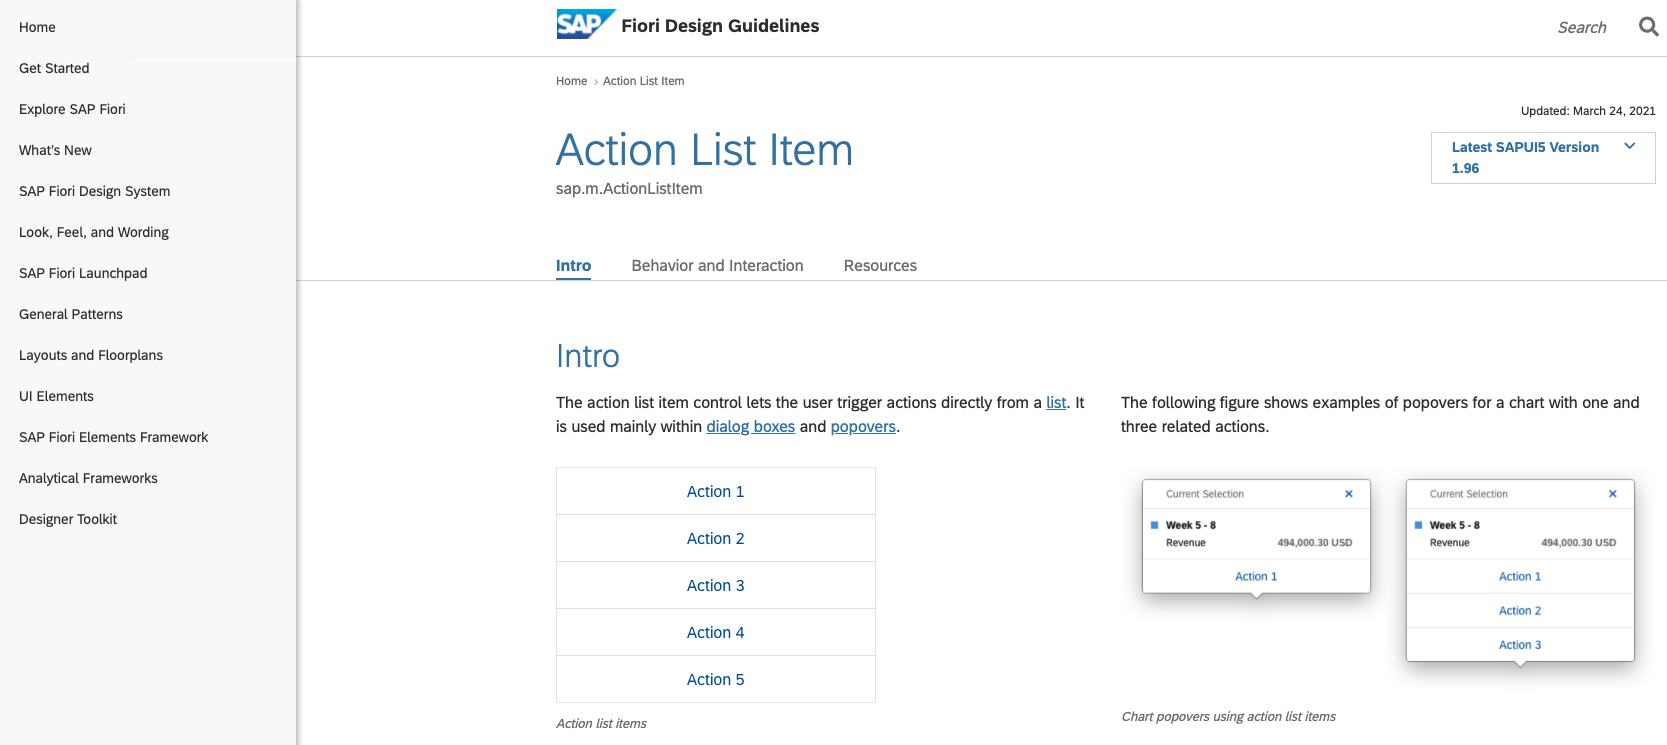
\includegraphics[width=\linewidth]{images/fiori_action-list_formal.png}}
\caption{SAP Fiori Action List formal guideline \cite{sap_fiori_nodate}}
\label{fiori_action_list}
\end{figure}
\newpage

\subsubsection{Usage guidelines} Usage guidelines help to understand how to use components. In addition, these guidelines explain how the corresponding parameters of a component work. This way, the user knows everything he needs to use the component in the product. \cite{vesselov_building_2019} \\
As in Figure \ref{atlassian_button}, the guidelines guide the users on where to implement the component. Sometimes usage guidelines also offer anti-patterns to the users. Anti-patterns tell users of the design system where they should not use that component.
\begin{figure}[htb]
\centerline{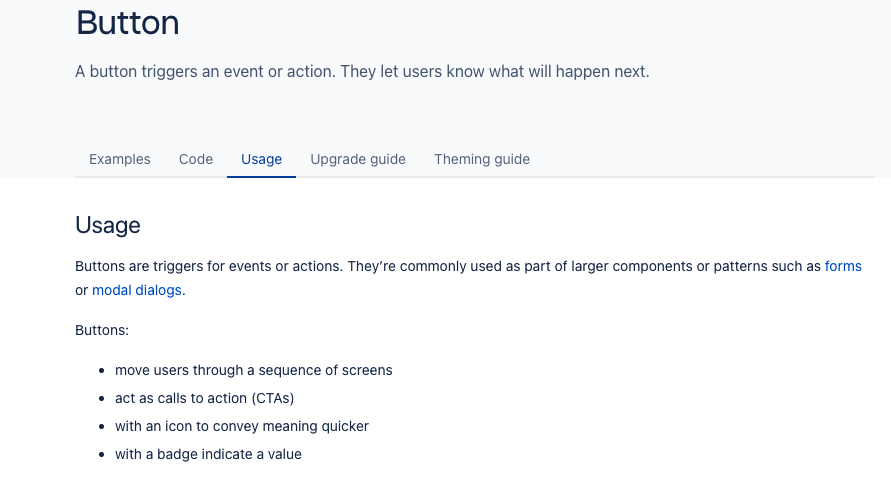
\includegraphics[width=\linewidth]{images/atlassian_button_usage.png}}
\caption{Atlassian Design System Button usage guideline \cite{atlassian_design_system_atlassian_nodate}}
\label{atlassian_button}
\end{figure}

\subsubsection{Technical guidelines} \label{tech_guideline}
\begin{wrapfigure}{r}{7cm}
	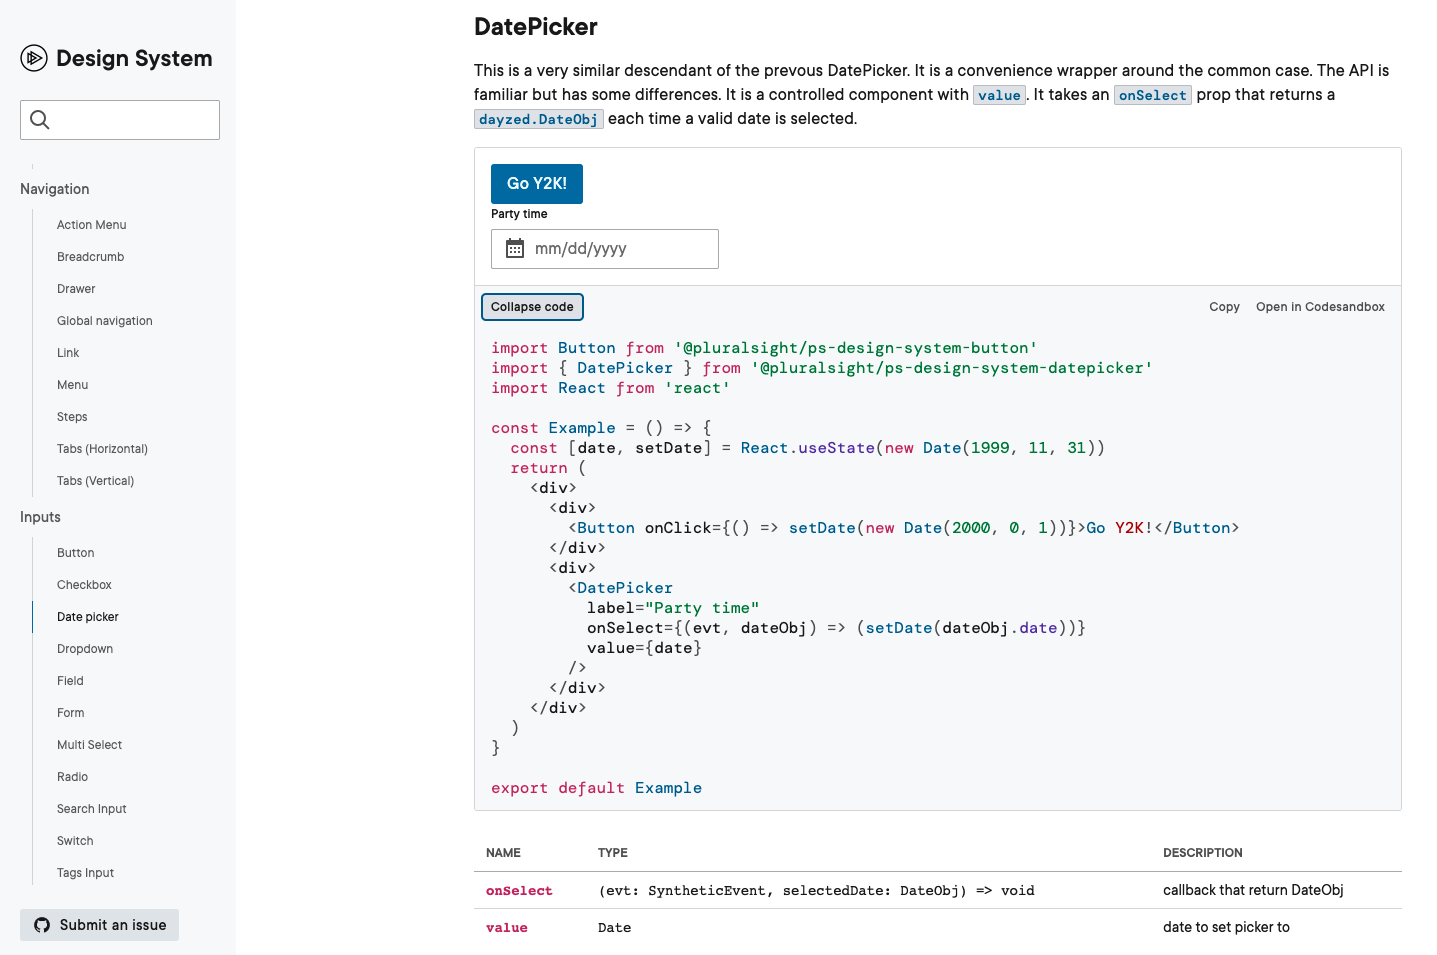
\includegraphics[width=7cm]{images/pluralsight_date-picker_technical.png}
	\caption{Pluralsight Design System Date picker technical guidelines \cite{pluralsight_ds_nodate}}
	\label{pluralsight_date_picker}
	\end{wrapfigure}
% Left here
Developers who implement the documented component in the software use this part of the documentation the most. Technical guidelines clarify ambiguities in implementation.  \cite{macdonald_practical_2019} \\
In the same way, the corresponding parameters configure the appearance or behavior of a component. An often-found feature here is copying code snippets. This functionality lets developers immediately copy and paste the component code into their code. \cite{vesselov_building_2019} \\
Figure \ref{pluralsight_date_picker} shows a good example.The implementation of Pluralsight's Date Picker is explained very well here with a code example. The code snippets can be copied directly, opened, and tried in a code sandbox.

\subsubsection{Related components} Linking components and patterns helps the user explore the design system. Also, this can support the creative process for designers and developers. \\
Figure \ref{servicenow_accordion} is an example of a linked component in a design system. Such a representation of a linked component helps with creativity and lets developers and designers move more quickly through the collection of components. \\
This way, if there are problems with the implementation, the developer can quickly understand the relationship between the used components and resolve the issue. \cite{vesselov_building_2019}
\begin{figure}[htbp]
\centerline{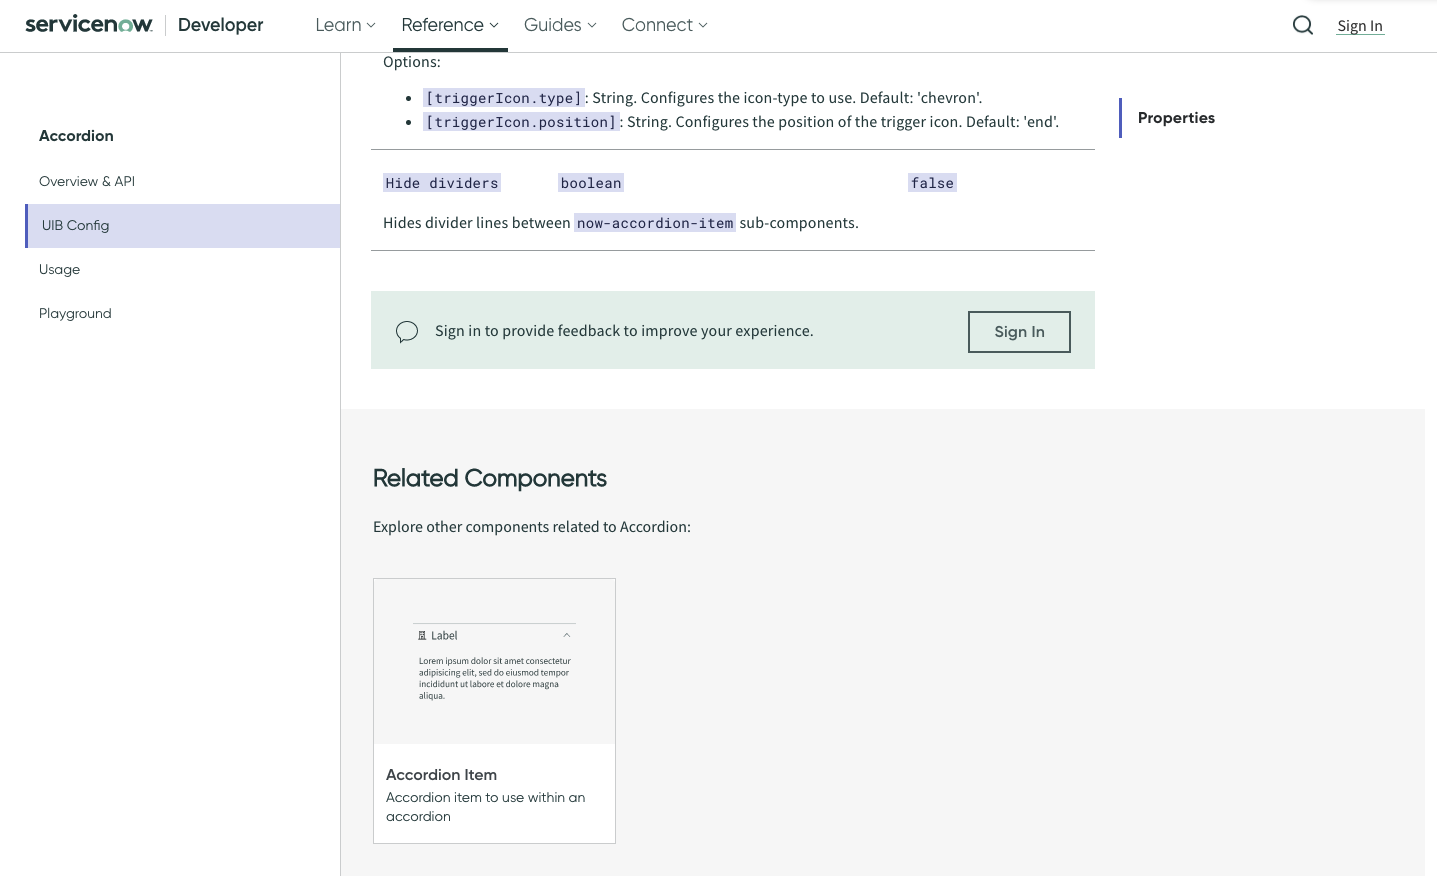
\includegraphics[height=150px]{images/servicenow_accordion_related.png}}
\caption{Servicenow Accordion related components \cite{servicenow_servicenow_nodate}}
\label{servicenow_accordion}
\end{figure}

\subsection{Design principles}\label{design_principles}
Design principles should be a central consideration when building a design system. At the same time, the design principles should reflect the norms and values of the product organization. In doing so, the points established do not follow any rules, except that they are set collectively by the team. \\
Thus, these design principles are a basis for design discussion and decision-making. By simply self-explanatory principles, the designers and developers can quickly create new designs without a significant coordination effort. Often questions are taken as principles. Questions give developers and designers the impulse to ask whether they follow the design principles during the creation process. \cite{brignell_design_2022} \\
As an example, \citet{berners-lee_principles_2013} has developed design principles for the web: 
\begin{itemize}
\item \textbf{Simplicity} - Simple solutions are better solutions
\item \textbf{Modular Design} - Change things, and it will only affect one part
\item \textbf{Being part of a Modular Design} - Realize you own the Design System
\item \textbf{Tolerance} - "Be liberal in what you require but conservative in what you do"
\item \textbf{Decentralization} - Do not produce bottlenecks; allow scaling in any direction
\item \textbf{Test of Independent Invention} - "Designing a system not to be modular in itself, but to be a part of an as-yet unspecified larger system."
\item \textbf{Principle of Least Power} - Use matching tools for the matching tasks
\end{itemize}
Design principles can be quite different. In this case, they are relatively technical, as the team wants to focus on this topic. Other organizations, such as Adobe with Adobe Spectrum, have people at the forefront. \cite{spectrum_adobe_spectrum_nodate} \\
Many underestimate the importance of these anchor points. Design principles play a central role in a design system.  The product team should build not only software based on these principles but also gain an understanding of the big picture of the product organization.  Therefore, the companies' design strategy aligns with their design principles. In this way, not only is the existing product organization aligned with the design principles, but new employees can also use them to integrate themselves more quickly into the product organization. Design principles are practical when they serve as a guide for the creative process.\cite{vesselov_building_2019} \\
First and foremost, a team must create design principles. A single person should not establish design principles on his or her own, even if it is possible. Developing design principles as a large group reflects the creative thinking of everyone and helps align the entire company with these values. \\
Here, \citet{vesselov_building_2019} lay out a 5-step plan to iteratively create and continuously improve them. Figure \ref{design_principles_steps} summarizes these five steps:
\newpage


\begin{figure}[htbp]
\centerline{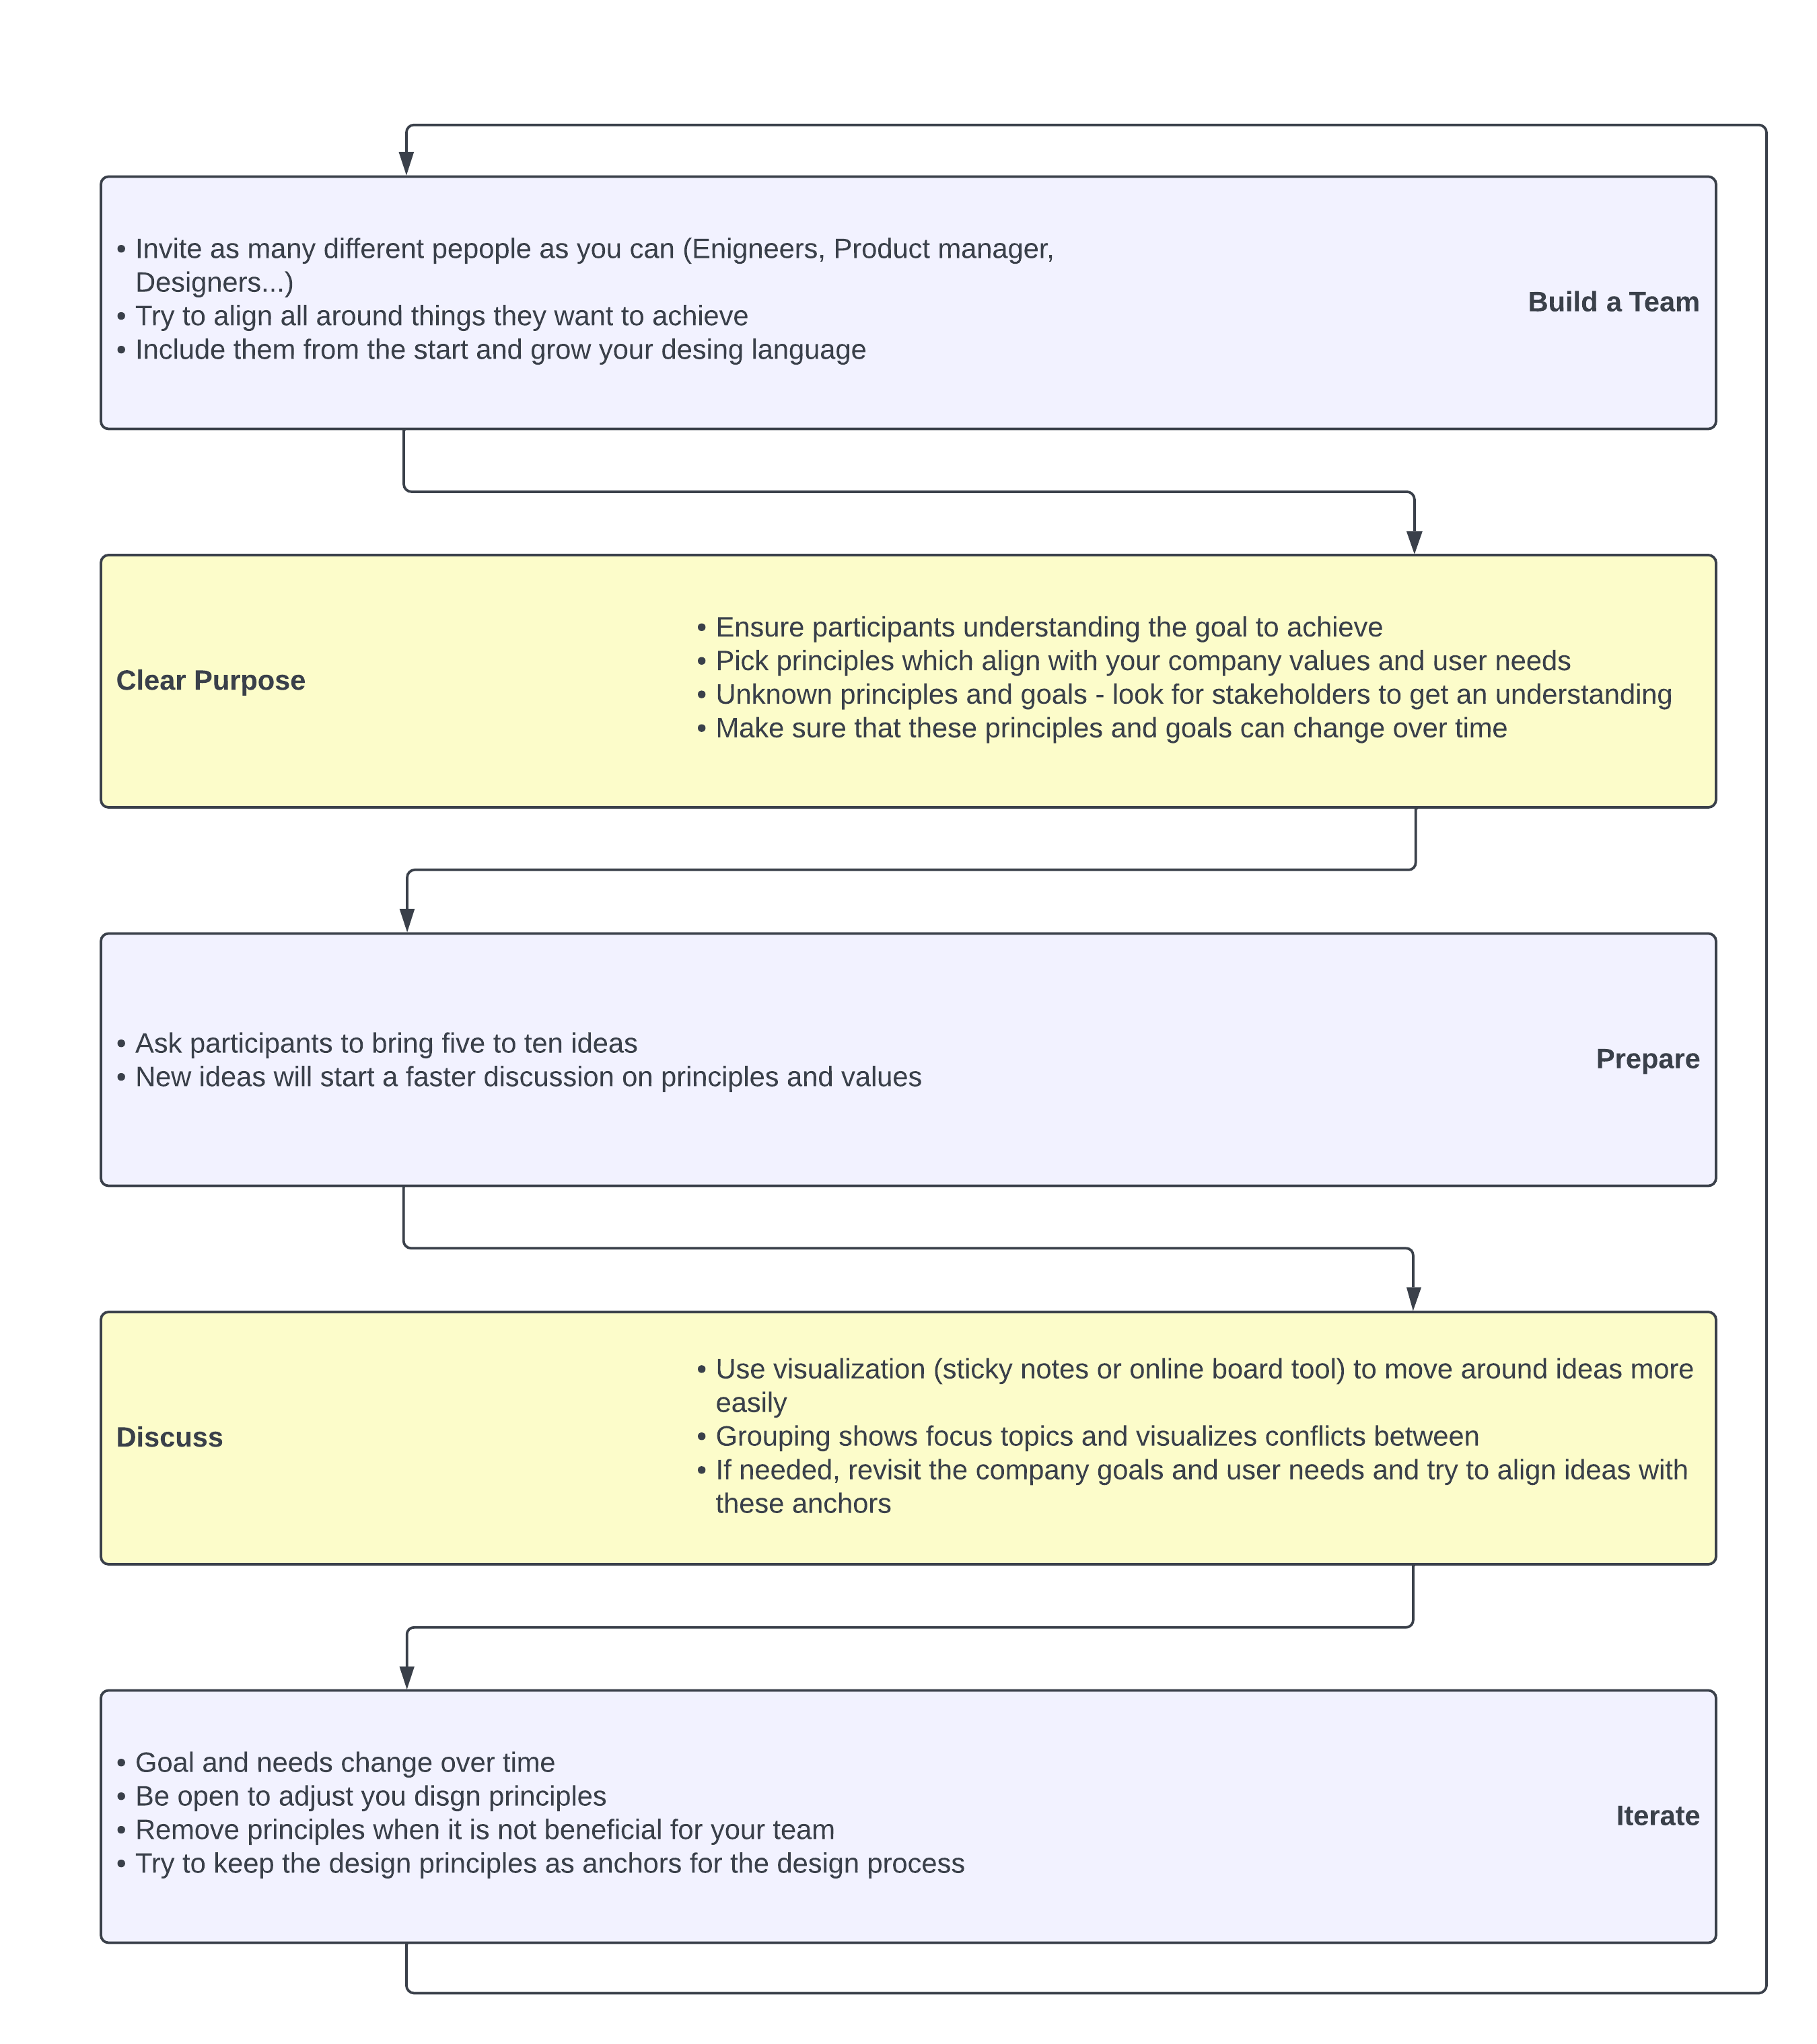
\includegraphics[width=\linewidth]{images/design_principles_steps.png}}
\caption{5 steps to introduce design principles inspired by  \citet{vesselov_building_2019}}
\label{design_principles_steps}
\end{figure}
Following these steps, a team creates design principles and implements an iterative process to update the design principles regularly. \\
Next, the responsible team shares the values of the created design principles with the rest of the product organization. Many design systems create so-called design blogs or design news in this step.  \\
They not only help the organization keep track of the design principles in their daily work. They also provide a platform to share updates with users. Moreover, there is an exchange on related topics on these platforms. A platform opens up communication, in turn, helps to improve and keep the design system and principles up to date.  \cite{google_material_2022} \\
This chapter lays the foundation with the guidelines and design principles, while the next chapter will introduce another building block: the component library.
\subsection{Component library}
The component library is the technical counterpart to the description guidelines and design principles. Both cannot exist in a design system without each other.  A component is “a constituent part” for, in this case, a user interface. \cite{component_definition} Combined with a library, a “collection of something”, it produces a collection of crucial constituent parts for user interfaces. \cite{library_definition} \\
The definitions existing from the literature are as follows:
\begin{tcolorbox}[title=Definition of a component library by \citet*{vesselov_building_2019}]
A set of styles and components that can be used and shared among a team. A component library consists of common core elements that are used throughout an application. [...] Component libraries may or may not include living code. [...] Unlike \ac{UI} frameworks such as Bootstrap, component libraries are tailored to specific purposes, like an internal brand.
\end{tcolorbox}
In addition to components, styling rules include layout specifications in component libraries. 
\begin{tcolorbox}[title=Definition of a component library by \citet*{macdonald_practical_2019}]
Component libraries, \ac{UI} libraries, or code libraries provide frontend code for \ac{UI} components (a.k.a. widgets, modules, chunks, blocks). Internally, you might use a component library as a shared collection of \ac{UI} snippets implementing patterns that anyone in the organization can contribute to building.
\end{tcolorbox}
An important point that emerges from these definitions is that component libraries focus on internal use. This argument is also the main difference between \ac{UI} frameworks. \\
After reviewing various design systems, four categories divide a component library: 
\begin{itemize}
	\item \textbf{Layout} - Spacing, and presentation of content placement on a site
	\item \textbf{Styles} - Color definitions, Typography, Icons
	\item \textbf{Components} - Reusable parts fulfilling one purpose
	\item \textbf{Patterns} - Combination of multiple components 
\end{itemize}

\subsubsection{Layout} \label{layout}
The foundation of any design system is the ability to place, move, or arrange elements on web pages. Applications achieve a consistent appearance by aligning spacing and positioning in a central place. \\ 
For this purpose, developers often use \ac{CSS} variables as design tokens. 
Like Tailwind (\url{https://tailwindcss.com/}), CSS classes implement design tokens and abstract them, so the developer does not need to use the variables natively. Thus, the developer does not need to know anything about \ac{CSS}.  \\
Salesforce Lightning Design System, for example, lists all layout tools under \textbf{Utilities}. It sets sizes for text, simple boxes, and spacing between components. They also have a sophisticated grid layout system.  \\
\begin{figure}[hbtp]
	\centerline{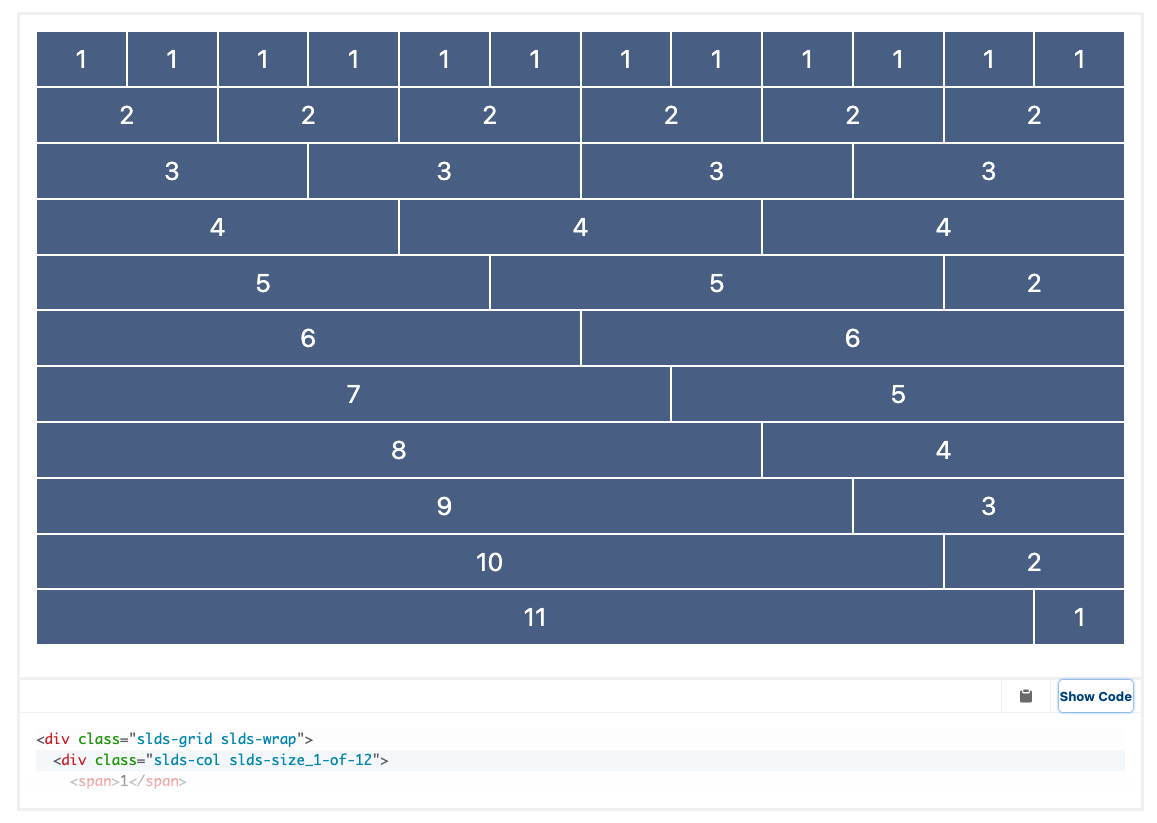
\includegraphics[width=\linewidth]{images/salesforce_lightning_layout.png}}
	\caption{Salesforce Lightning Design System grid layout \cite{lightning_design_system_lightning_nodate}}
	\label{salesforce_lightning_layout}
\end{figure} 

Figure \ref{salesforce_lightning_layout} shows that \ac{CSS} classes achieve the desired layout. Furthermore, both dynamic and static layouts are supported. So the user has all possibilities to use the layout of the design system.\\
Besides the usual spacing and positioning regulations, the layout also describes other points like visibility, scroll ability, or printability. The default layouting in the design system specifies all requirements for visible elements in the target system.

\subsubsection{Styles}
Styles are about colors, typography, and icons. These topics may seem trivial, but it is vital to make a connection to the chosen design principles. In addition, this helps to convey that design language in the other disciplines of the component library. \\
A style system provides enough freedom for design decisions so that the implemented products can still have a unique look and feel. Some component libraries ensure this by allowing customization of basic style parameters.\cite{vesselov_building_2019}

\paragraph{Color}
An excellent first step is introducing a color system to build a design system. Colors are essential for the aesthetics of a product.
Without changing the functionality or layout, the product team can change the colors until they fit the product. \\
\begin{figure}[htbp]
	\centerline{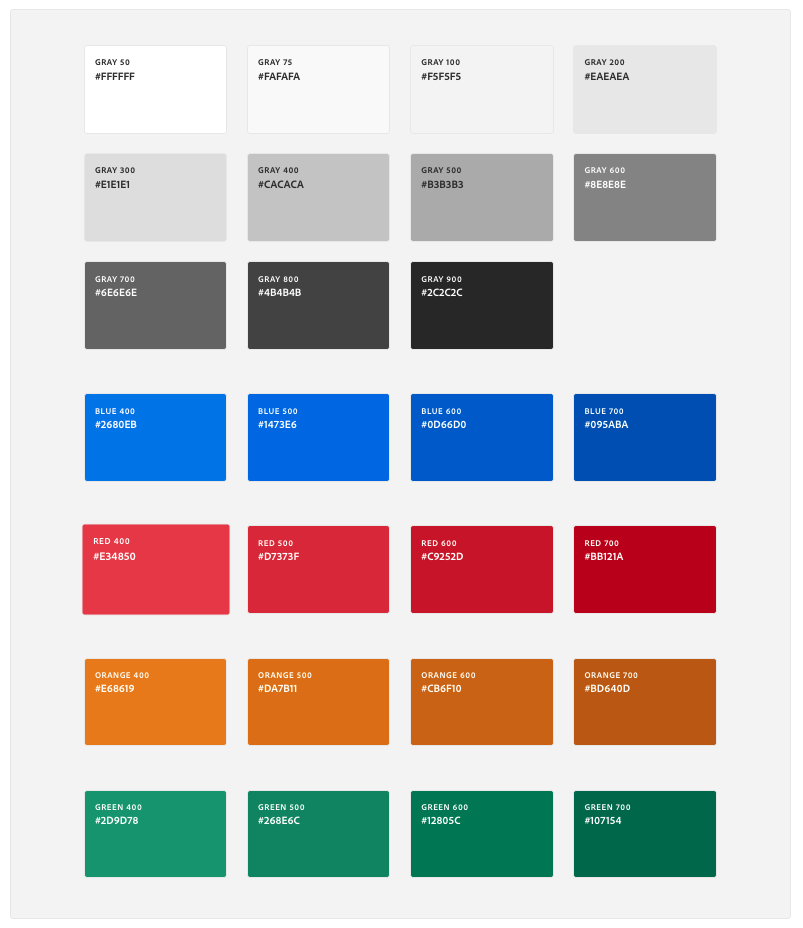
\includegraphics[height=8cm]{images/adobe_spectrum_color_palette.png}}
	\caption{Adobe Spectrum color palette \cite{spectrum_adobe_spectrum_nodate}}
	\label{adobe_spectrum_colors}
\end{figure}
It is always fundamental to keep accessibility in mind when choosing colors. For a specific text size, it is necessary to maintain a particular contrast on colors. The WCAG (\url{https://www.w3.org/WAI/standards-guidelines/wcag/}) describes this contrast with two levels, AA and AAA. This contrast is especially significant if a product has several long paragraphs.  \\
Adobe's Spectrum Design System in Figure \ref{adobe_spectrum_colors} illustrates that design systems provide not just one color but an entire color palette. The palette divides colors often into primary, secondary, text color, background color, accent colors, shadows, and many more. \\
Again, \ac{CSS} variables with the appropriate names consume color tokens to provide them later for product implementation. The challenge is to offer a well-defined color palette but at the same time not overload the user. Too many colors quickly confuse users about which color to use for the feature. \cite{vesselov_building_2019}

\paragraph{Typography}
A typography system has two different categories. \\
First, there is typography for smaller text elements. Such elements consist of a maximum of three words. Examples are headings, buttons, or labels. \\
Second, typography determines the appearance of long paragraphs. For example, paragraphs can have a different weight, size, or font family. 
\begin{figure}[hbtp]
	\centerline{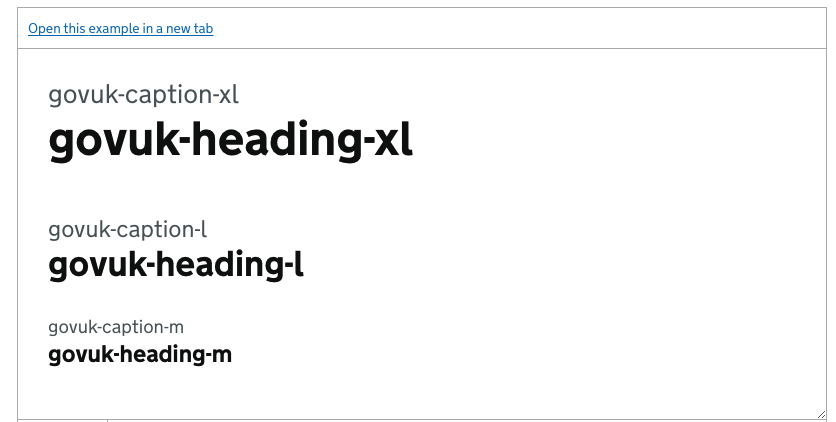
\includegraphics[height=5cm]{images/gov_uk_typo.png}}
	\caption{GOV.UK Design System caption typography example \cite{govuk_govuk_nodate}}
	\label{gov_uk_typo}
\end{figure} \\
In both cases, however, the general typography must follow the defined layout system. Texts rely on defined design features for spacing and padding. Figure \ref{gov_uk_typo} shows a helpful tool, an overview of all typography options supports the selection of the right design.  \cite{vesselov_building_2019}


\paragraph{Iconography}
Iconography is a bit of a specialty in a design system. It may not seem necessary for a product, but icons often deliver a lot of the overall design language to the end user. \\
Although icons are essential to design language, creating new iconography is not always necessary. A good start is to use an iconography that is already widely used. Later, a custom iconography offers much potential to visualize the company’s design language. \\
As with other parts of a design system, documentation is key. Next, focus on how to create new icons and what proportions and shapes. If done right, it is an easy step to introduce new icons into the iconography. 
\\
An iconography describes adding icons to the product to make icons accessible to the team. As in the technical guidelines in \ref{tech_guideline}, a code snippet explains their use to the developer. \cite{vesselov_building_2019}

\subsubsection{Components}
Components are the heart of a component library and the building blocks for every application. All the tools and fundamentals just presented together build components. Components are highly reusable and as flexible.  \\
\begin{figure}[hbtp]
	\centerline{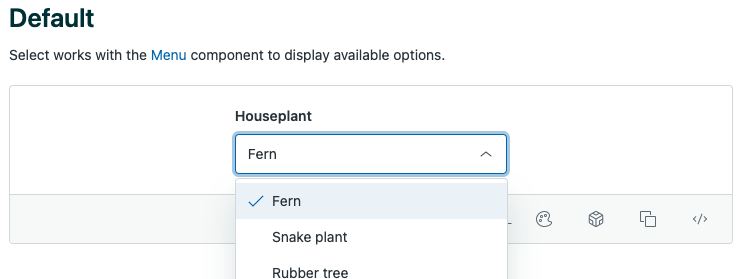
\includegraphics[height=5cm]{images/zendesk_component_example.png}}
	\caption{Zendesk Garden dropdown component \cite{zendesk_garden_zendesk_nodate}}
	\label{zen_garden_component}
\end{figure}

Combinations of layout and style specifications result in components for different use cases. Also, Figure \ref{zen_garden_component} shows a dropdown component. Many different design systems implement that kind of component.Because native dropdowns often cannot meet complete user experience requirements, component libraries have often replicated this component. \\
By using these predefined components in applications, the developer ensures that the guidelines adhere too.For certain combinations of components in an application, there is another term called patterns, and chapter \ref{patterns} will explain them in more detail. \\

\begin{figure}[hbtp]
	\centerline{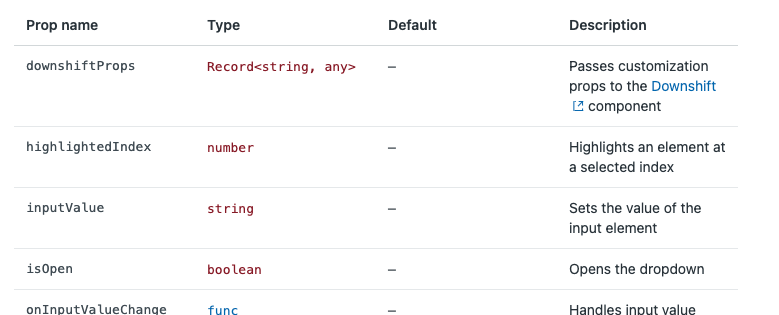
\includegraphics[height=5cm]{images/zendesk_component_interface.png}}
	\caption{Zendesk Garden dropdown interface \cite{zendesk_garden_zendesk_nodate}}
	\label{zen_garden_interface}
\end{figure}
It is essential to always have the component’s interfaces in mind to achieve flexibility and reusability. Well-defined interfaces are the key to successful components. A possible solution, as in Figure \ref{zen_garden_interface}, is good interface documentation. A simple table with property values, the expected type, and a short description is sufficient. In some design systems, the developer can change these input properties in a live demo so that the developer can see the changes immediately.\\
As with other parts of a design system, documentation is key. To get well-documented interfaces, always involve the engineers who are building the product to receive their feedback.  A well-structured and systematic approach to how a component work helps developers use the components.  \cite{vesselov_building_2019}\\
The components mentioned above alone are not enough. Sometimes it takes more than one component to get the job done. The next chapter explains how patterns achieve documentation of a complex component construct. 

\subsubsection{Patterns} \label{patterns}
A combination of specific components is often used repeatedly in different places and applications. For this, a design system has a concept called patterns.\\ 
Patterns specify a combination of several components and document the composition of these components. Patterns are extended documentation to reproduce a particular combination of components in an application. \\
\begin{figure}[htbp]
	\centerline{
\includegraphics[height=7.5cm]{images/atlassian_abstract_form.png}}
	\caption{Atlassian Design System abstract form layout \cite{atlassian_design_system_atlassian_nodate}}
	\label{atlassian_form_layout}
\end{figure}
Atlassian's design system provides an excellent example of a pattern with its forms. Figure \ref{atlassian_form_layout} illustrates how a form places input fields and buttons on a single page. This abstraction leaves no room for interpretation, and developers and designers can continue their work. \\
Patterns refer not only to the interaction of components but also to the switching of visualization due to changes in a user's permissions, for example. A pattern documents all \ac{UI} changes related to the user experience, no matter how small. \cite{vesselov_building_2019} \\
Most often, patterns appear in the general navigation of applications. Such navigation patterns evolve naturally from an introduction to products and grow iteratively with more and more feedback from the product development team. \\
An excellent example of a pattern is the navigation bar. A navigation bar is created by combining components such as buttons, dropdowns, and images. Together with skeleton code around these components documented in a pattern, they form a complete navigation area within an application. 
